% Citadel-Rx manuscript. Compile: pdflatex main (IEEEtran, TikZ). Figures: ../docs/figures.
% Every number is regenerated from the JSON records in results/ by the scripts named in the
% captions (docs/RESULTS.md, docs/STATS.md, docs/TABLES.md). Nothing is typed from memory.
\documentclass[journal]{IEEEtran}
\usepackage{amsmath,amssymb,amsthm,bm}
\usepackage{graphicx}
\usepackage{booktabs,multirow,array}
\usepackage{tikz}
\usetikzlibrary{arrows.meta,positioning,shapes.geometric,fit,calc}
\usepackage[hidelinks]{hyperref}
\usepackage{cite}
\usepackage{url}
\graphicspath{{../docs/figures/}}

\newtheorem{theorem}{Theorem}
\newtheorem{lemma}{Lemma}
\newtheorem{proposition}{Proposition}
\newtheorem{assumption}{Assumption}
\newcommand{\norm}[1]{\left\lVert #1 \right\rVert}
\newcommand{\E}{\mathbb{E}}
\tikzset{box/.style={draw,rectangle,align=center,font=\scriptsize,inner sep=3pt,minimum height=5.5mm},
         dbox/.style={box,dashed},
         arr/.style={-{Latex[length=1.6mm]},thin},
         darr/.style={-{Latex[length=1.6mm]},thin,dashed},
         lbl/.style={font=\tiny,fill=white,inner sep=1pt}}

\begin{document}

\title{Citadel-Rx: Continuum-Memory Test-Time Learning for Neural Receivers With Physics-Gated Consolidation Against Pilot Poisoning}

\author{Abraheem~Rashid%
\thanks{A. Rashid is with the Department of Computer Science, Brunel University London, London, U.K. (e-mail: 2546393@brunel.ac.uk).}%
\thanks{Code, configuration, every run record and the scripts that regenerate every table and figure: \url{https://github.com/abraheemrashid99-sys/Citradel-Rx}.}}

\markboth{IEEE Transactions on Wireless Communications}{Rashid: Citadel-Rx}
\maketitle

\begin{abstract}
Neural receivers that learn at test time adapt to the channel from the pilots of every
coherence block, so the pilot stream is a training set that an adversary can write to. A
perturbation shaped through the receiver's own adaptation step and injected on the pilots
destroys online and meta-learned DeepSIC receivers, and meta-learning keeps the poison.
We propose Citadel-Rx, a DeepSIC receiver whose adaptable parameters are kept at three
nested time-scales: a fast level fitted on every block, and two slow levels updated every
8 and 32 blocks through a gated average of the faster states. Three label-free
physics-consistency gates, each a ratio against a model-based reference on the same
block, decide what may be consolidated: a residual test against the linear channel
model, a CRC pass-rate test whose threshold follows from the post-adaptation symbol
error probability, and an innovation test against the channel prior. A rejected block is
reverted and its data are detected with the slow memory. We prove, for the algorithm as
implemented, that the displacement a budget-$\epsilon$ attack causes in the slowest level
over $W$ blocks is bounded by the fast level's displacement times
$1-(1-\eta^{(K)})^{\lceil W/C_K\rceil}$, and check the bound with measured constants. In
1\,926 recorded runs over four channel families, $4\times4$ and $8\times8$ systems, three
Doppler rates and five attackers, Citadel-Rx keeps its clean symbol error rate at every
budget from $-10$ to $+10$\,dB signal-to-interference ratio (attack-window SER
$0.026$--$0.034$ against $0.28$--$0.97$ for online DeepSIC and $0.24$--$0.86$ for
Meta-DeepSIC, all paired differences significant after Holm correction), rejects
$86$--$99\%$ of poisoned blocks with at most $1.7\%$ false rejections, and, without any
attack, halves the SER of online DeepSIC at 10\,dB because the slow memory acts as a
prior for the per-block fit. Ablations attribute the clean gain to the proximal anchor
and the robustness to the slow memory and the fallback. The evaluation also reports where
the defence is weakest: at symbol error rates near $10^{-4}$ the few poisoned blocks that
pass the gate set a floor near $10^{-3}$, and on a nearly diagonal channel the clean gain
over LMMSE vanishes.
\end{abstract}

\begin{IEEEkeywords}
Deep receivers, test-time learning, adversarial pilot poisoning, meta-learning, continual
learning, physics-informed gating, MIMO detection, 6G security.
\end{IEEEkeywords}

\section{Introduction}
\IEEEPARstart{D}{eep} receivers replace or augment the model-based blocks of a MIMO
detector with neural networks trained on data \cite{oshea2017,honkala2021,samuel2019,
shlezinger2023}. Because a network trained in simulation meets a different channel in
the field, the strongest of them adapt at test time: online DeepSIC
\cite{shlezinger2021} re-trains its per-user networks on the pilots of every coherence
block, and Meta-DeepSIC \cite{raviv2023} meta-learns an initialisation from the pilots
of past blocks so that the per-block fit converges faster. Their adaptation data are the
only labelled symbols the receiver ever sees: a few hundred pilot bits per user per
block.

The security problem addressed here is the following. An adversary within range of the
base station adds a perturbation to the received pilot part of a block, with an energy
budget expressed as a signal-to-interference ratio (SIR) over the pilots. Wu
\emph{et al.} \cite{wu2024} showed that a perturbation shaped through an unrolled copy
of the receiver's adaptation step raises the post-adaptation symbol error rate (SER) of
online DeepSIC by an order of magnitude, that a perturbation crafted on a surrogate
receiver still transfers, and that Meta-DeepSIC, which keeps the poisoned pilots in its
support set, does not recover after the attack stops. They call for receivers that are
secure by construction. We are not aware of one. Four properties of the problem shape our
design and its evaluation. First, the receiver cannot verify its adaptation data: the
pilots are the labels. What it can verify is physical consistency: whether its
decisions fit a linear channel model, whether the CRC of the decoded data passes, and
whether the estimated channel moved as a channel does. Second, the harm of poisoning is
not in the attacked block alone but in what the receiver keeps: a defence must protect
the memory, not only the decision. Third, an attacker who knows the defence will try to
pass its tests, so the tests must be tied to the attacker's own objective. Fourth, the
value of a defence can only be established against the attacks of the literature, under
the same channel realisations as the baselines, over many seeds, with the clean cost of
the defence reported alongside its benefit.

\begin{table}[t]
\centering\caption{Positioning by method class (--: not addressed; the attack surface is
what the adversary can write to).}\label{tab:pos}
\scriptsize
\begin{tabular}{@{}lllll@{}}
\toprule
Class & Adapts & Memory & Attack surface & Defence\\
\midrule
LMMSE & no & -- & pilot estimate & --\\
Online DeepSIC \cite{shlezinger2021} & every block & last block & pilots & --\\
Meta-DeepSIC \cite{raviv2023} & every block & pilot buffer & pilots, persistent & --\\
Drift-detection receiver & on drift & last block & pilots & adapt less\\
Robust TTA (vision) \cite{medbn,wu2023tta} & every batch & batch stats & batch & robust statistics\\
Byzantine aggregation \cite{blanchard2017} & -- & -- & gradients & needs many vectors\\
Nested / continuum memory \cite{behrouz2025nested,behrouz2025titans} & every token & multi-rate & input & --\\
Citadel-Rx (ours) & every block & 3 rates, gated & pilots & physics gates, certified retention\\
\bottomrule
\end{tabular}
\end{table}

Prior work addresses these properties separately (Table~\ref{tab:pos}). Test-time
adaptation in vision has its own poisoning problem \cite{wu2023tta}, and its defences
replace batch statistics or gradients by robust estimates \cite{medbn}; they assume
i.i.d. batches and, as we show, do not transfer to a receiver that sees one correlated
block at a time. Byzantine-robust aggregation \cite{blanchard2017} needs many gradient
vectors per step, which a receiver with one pilot block does not have. Certified
defences against data poisoning \cite{steinhardt2017} bound the loss of a convex learner
under a fraction of corrupted points; our setting is sequential, the learner is a
network, and the corruption is a bounded perturbation of every point in a block.
Corruption-robust online learning \cite{lykouris2018} gives the additive accounting we
use. Nested learning \cite{behrouz2025nested} and Titans \cite{behrouz2025titans} keep
memory at several update frequencies; they do not decide what enters the slow memory,
and a single test-time memory is, as our ablation shows, as vulnerable as online
DeepSIC. Table~\ref{tab:pos} summarises the gap: no published receiver keeps memory at
several rates, gates what enters the slow rates on physics the attacker cannot forge
without giving up its objective, and comes with a retention guarantee checked against
measurements.

The contributions of this paper are as follows.
\begin{enumerate}
\item \textbf{A three-timescale receiver} (Section~\ref{sec:citadel}): a fast level with
a delta-rule learner and a surprise-generated step size, slow levels at periods aligned
with the channel's coherence structure, gated consolidation, a proximal anchor that pulls
the fast level toward the slow projection, and a gated fallback that detects a rejected
block with the uncorrupted memory.
\item \textbf{Relative physics gates} (Section~\ref{sec:gates}): three label-free tests
whose statistics are ratios against a model-based reference computed on the same block,
so that a channel that merely degrades does not look like a poisoned adaptation. The CRC
gate's threshold is derived, not tuned, from a target excess SER
(Proposition~\ref{prop:crc}), and a relative slack keeps it meaningful at $10^{-3}$
operating points.
\item \textbf{A retention certificate for the implemented algorithm}
(Section~\ref{sec:theory}): the slowest level's exposure to a bounded attack is divided
by its period and multiplied by the gate's miss rate (Theorem~\ref{thm:cert}), with a
regret decomposition in which the adversary's term is additive
(Theorem~\ref{thm:regret}). Every constant is measured; the bound is drawn against
paired adversarial/clean memory trajectories.
\item \textbf{A reproducible, paired evaluation} (Sections~\ref{sec:setup}--\ref{sec:results}):
seven receivers, five attackers, four channel families, two system sizes, three Doppler
rates, three to five seeds; bootstrap intervals and Holm-corrected Wilcoxon tests on
per-block differences paired on the channel realisation; every number regenerated from
1\,926 recorded runs by one script each.
\end{enumerate}
The evaluation also reports where the defence does \emph{not} help: where the clean SER is
near $10^{-4}$ the attacked window sits near $10^{-3}$ because the few poisoned blocks
that pass the gate dominate; on a nearly diagonal channel the clean gain over LMMSE
vanishes; and the first calibration of the relative CRC slack raised false rejections to
$15$--$20\%$ before it was corrected. We attribute the controller's advantages to its
individual components in Section~\ref{sec:ablate}.

Section~\ref{sec:model} presents the system and threat model, Section~\ref{sec:citadel}
the receiver, Section~\ref{sec:theory} the guarantees, Section~\ref{sec:setup} the
experimental setup, Sections~\ref{sec:results} and \ref{sec:discussion} the results and
their scope, and Section~\ref{sec:conclusion} concludes.

\section{System Model and Threat Model}\label{sec:model}
We first fix the uplink, the receiver that is attacked, the attacker, and the metrics by
which every method is judged.

\subsection{Uplink and Adaptive Receiver}
$U$ single-antenna users transmit QPSK symbols to a base station with $N$ antennas. Time
is divided into coherence blocks $b=1,2,\dots$; within block $b$ the channel $\bm
H_b\in\mathbb{C}^{N\times U}$ is constant and the received vector at symbol slot $n$ is
\begin{equation}\label{eq:channel}
\bm y_n = f\!\left(\bm H_b \bm s_n\right)+\bm w_n,\qquad \bm w_n\sim\mathcal{CN}(\bm 0,\sigma^2\bm I),
\end{equation}
with $f$ the identity (linear channel) or the memoryless power-amplifier nonlinearity
$f(x)=\tanh(0.5x)$ applied per antenna, as in \cite{raviv2023}. Each block carries $N_p$
pilot symbols per user, known to the receiver, followed by $N_d$ data symbols framed in
CRC-protected sub-blocks of $L$ symbols (Table~\ref{tab:setup}). Four channel families
are used (Section~\ref{sec:setup}).

\begin{table}[t]
\centering\caption{Simulation setup, read from the configuration files and the code.}
\label{tab:setup}
\scriptsize
\begin{tabular}{@{}ll@{}}
\toprule
Item & Value\\
\midrule
System & $U\times N=4\times4$ (Sec.~\ref{sec:gen}: $8\times8$), QPSK, SNR $10$\,dB (swept $4$--$16$)\\
Block & $N_p=100$ pilot symbols (200 bits), $N_d=25\,000$ data symbols per user\\
CRC & CRC-8 (3GPP polynomial \cite{ts38212}), $L=32$ symbols per sub-block, $n=781$ sub-blocks\\
Channel & SED $[\bm H]_{ij}=e^{-|i-j|}$ with per-user cosine fading (periods 51/39/33/21, depth 0.8) \cite{shlezinger2021};\\
        & Jakes block correlation $\rho=J_0(2\pi f_DT_b)$, $f_DT_b\in\{0.01,0.05,0.1\}$ \cite{jakes1974};\\
        & $\tanh$ PA nonlinearity; COST2100 traces of \cite{raviv2023} \cite{liu2012cost}\\
Run & 100 blocks (400 for A3), attack on blocks 30--69, seeds 0--2 (0--4 on headline cells)\\
DeepSIC & $Q=3$ iterations, per-user MLP $64\cdot$order hidden units, ReLU \cite{shlezinger2021}\\
Adaptation & Adam, lr $5\cdot10^{-3}$, 300 epochs per block on the pilots; joint pre-training at 2--16\,dB\\
Attacker & PGD, 20 steps, step $0.25\,\epsilon$, 2 unrolled adaptation steps \cite{wu2024,madry2018}\\
\bottomrule
\end{tabular}
\end{table}

The receiver is DeepSIC \cite{shlezinger2021}: $Q$ soft-interference-cancellation
iterations, each a per-user multilayer perceptron that maps the received vector and the
other users' current soft decisions to a posterior over the user's symbol. Its
parameters $\theta$ are adapted on the pilots of every block,
\begin{equation}\label{eq:adapt}
\theta_b=\Phi(\theta_{b-1};\bm Y_b),
\end{equation}
by $T$ steps of a first-order optimiser on the pilot cross-entropy, and then detect the
data of the block. Online DeepSIC starts every block from $\theta_{b-1}$; Meta-DeepSIC
starts from an initialisation meta-learned by MAML \cite{finn2017} on a buffer of past
pilot blocks, refreshed every five blocks \cite{raviv2023}.

\subsection{Threat Model}
The adversary adds $\bm E_b$ to the received pilot matrix $\bm Y_b\in\mathbb{C}^{N\times
N_p}$ of block $b$, with $\norm{\bm E_b}_F\le\epsilon_b$ set by the SIR over the pilot
block,
\begin{equation}\label{eq:budget}
\epsilon_b=\norm{\bm Y_b}_F\,10^{-\mathrm{SIR}/20},
\end{equation}
so that SIR $0$\,dB spends as much energy as all $U$ users together; the data part is not
touched. The attacker knows the pilots (they are standardised) and sees the channel
through its own receiver. Following and extending \cite{wu2024} we consider:
\begin{itemize}
\item \emph{A1, availability.} Projected gradient ascent \cite{madry2018} on the
post-adaptation data loss, differentiated through an unrolled copy of the victim's
adaptation map \eqref{eq:adapt} (white-box), or crafted on a surrogate online DeepSIC
and injected (transfer). A receiver without an adaptation map (LMMSE) is attacked through
the surrogate.
\item \emph{A2, targeted drift.} A1 with an objective that raises one user's loss while
keeping the others' low, on a Jakes channel, so that the poison looks like a plausible
channel change.
\item \emph{A3, boiling frog.} Many blocks of small perturbations ($5\%$ of the pilot
energy) that push the receiver toward a spoofed channel basin while keeping the SER
inside any tolerance a detector might use.
\item \emph{Adaptive, gate-aware.} A1 with a penalty on the defence's gate statistics in
the attacker's objective: an attacker who knows the defence and tries to pass it.
\end{itemize}
A \emph{data-jamming control} spends the same energy on the data part of the block
instead of the pilots; it separates persistent poisoning from plain interference.

\subsection{Metrics}
We report the SER as the fraction of symbol slots in which at least one user is wrong,
the metric of \cite{shlezinger2021,raviv2023,wu2024}, as a mean over the attack window
(blocks 30--69), before it (pre) and after it (post); the recovery time, the number of
blocks after the attack until the 3-block moving average returns within $10\%$ of the
pre-attack mean (30 = not within the run); the gate's rejection rate of poisoned blocks
and false-rejection rate of clean blocks; the degradation $\Delta_{\rm dB}$, the extra
SNR needed under attack to reach the clean SER \cite{wu2024}; and the paired displacement
$D_k(W)=\norm{\theta^{(k)}_{\rm adv}-\theta^{(k)}_{\rm clean}}$ of memory level $k$ between
an attacked and a clean run on the same channel. Fig.~\ref{fig:pipeline} summarises the
study from configuration to every reported number.

\begin{figure}[t]
\centering
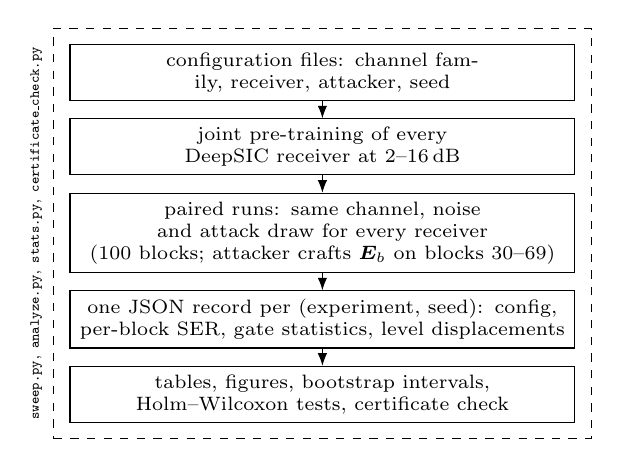
\begin{tikzpicture}[node distance=2.2mm]
\node[box,text width=62mm] (a) {configuration files: channel family, receiver, attacker, seed};
\node[box,text width=62mm,below=of a] (b) {joint pre-training of every DeepSIC receiver at 2--16\,dB};
\node[box,text width=62mm,below=of b] (c) {paired runs: same channel, noise and attack draw for every receiver\\ (100 blocks; attacker crafts $\bm E_b$ on blocks 30--69)};
\node[box,text width=62mm,below=of c] (d) {one JSON record per (experiment, seed): config, per-block SER, gate statistics, level displacements};
\node[box,text width=62mm,below=of d] (e) {tables, figures, bootstrap intervals, Holm--Wilcoxon tests, certificate check};
\draw[arr] (a)--(b); \draw[arr] (b)--(c); \draw[arr] (c)--(d); \draw[arr] (d)--(e);
\node[dbox,fit=(a)(e),inner sep=2mm] (f) {};
\node[lbl,rotate=90,anchor=south] at ($(f.west)+(-1mm,0)$) {\texttt{sweep.py}, \texttt{analyze.py}, \texttt{stats.py}, \texttt{certificate\_check.py}};
\end{tikzpicture}
\caption{Study pipeline from configuration to every reported number; finished records are
skipped on re-run, so every stage is resumable.}
\label{fig:pipeline}
\end{figure}

\section{Citadel-Rx}\label{sec:citadel}
The receiver splits adaptation by time-scale: a fast level fits every block; slow levels
are updated at the periods of the channel's coherence structure, and only with what the
gates accept. Fig.~\ref{fig:arch} shows the architecture.

\begin{figure*}[t]
\centering
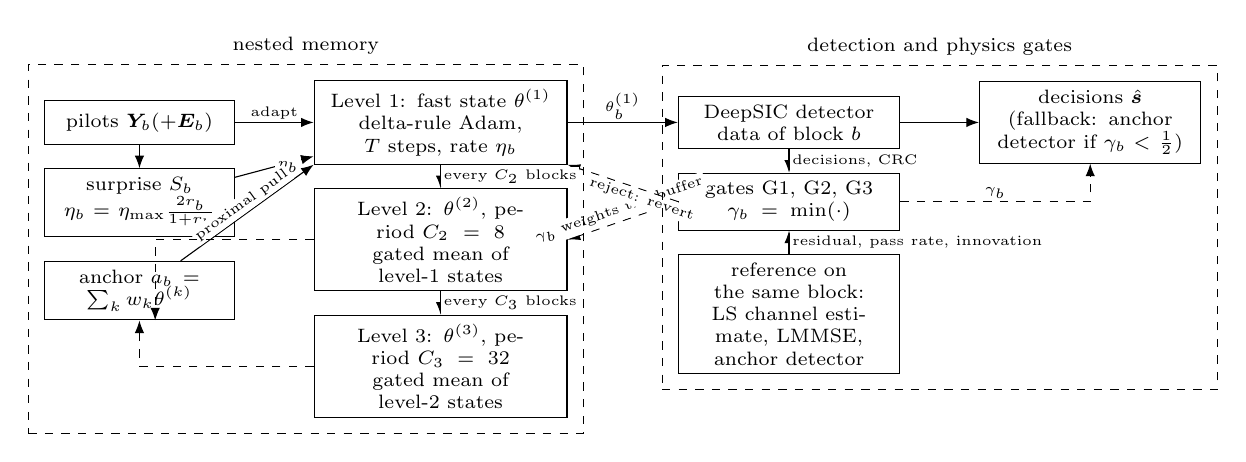
\begin{tikzpicture}[node distance=3mm and 6mm]
\node[box,text width=30mm] (fast) {Level 1: fast state $\theta^{(1)}$\\ delta-rule Adam, $T$ steps, rate $\eta_b$};
\node[box,text width=30mm,below=of fast] (l2) {Level 2: $\theta^{(2)}$, period $C_2=8$\\ gated mean of level-1 states};
\node[box,text width=30mm,below=of l2] (l3) {Level 3: $\theta^{(3)}$, period $C_3=32$\\ gated mean of level-2 states};
\node[box,text width=26mm,right=14mm of fast] (det) {DeepSIC detector\\ data of block $b$};
\node[box,text width=26mm,below=of det] (gate) {gates G1, G2, G3\\ $\gamma_b=\min(\cdot)$};
\node[box,text width=26mm,below=of gate] (ref) {reference on the same block:\\ LS channel estimate, LMMSE, anchor detector};
\node[box,text width=22mm,left=10mm of fast] (pil) {pilots $\bm Y_b(+\bm E_b)$};
\node[box,text width=22mm,below=of pil] (sur) {surprise $S_b$\\ $\eta_b=\eta_{\max}\frac{2r_b}{1+r_b}$};
\node[box,text width=22mm,below=of sur] (anc) {anchor $a_b=\sum_k w_k\theta^{(k)}$};
\node[box,text width=26mm,right=10mm of det] (out) {decisions $\hat{\bm s}$\\ (fallback: anchor detector if $\gamma_b<\tfrac12$)};
\draw[arr] (pil)--(fast) node[midway,lbl,above]{adapt};
\draw[arr] (pil)--(sur); \draw[arr] (sur)--(fast) node[midway,lbl,right]{$\eta_b$};
\draw[arr] (anc)-- (fast.south west) node[midway,lbl,above,sloped]{proximal pull};
\draw[arr] (fast)--(det) node[midway,lbl,above]{$\theta^{(1)}_b$};
\draw[arr] (det)--(out);
\draw[arr] (det)--(gate) node[midway,lbl,right]{decisions, CRC};
\draw[arr] (ref)--(gate) node[midway,lbl,right]{residual, pass rate, innovation};
\draw[darr] (gate.west)-- (l2.east) node[midway,lbl,above,sloped]{$\gamma_b$ weights the buffer};
\draw[darr] (gate.west)-- (fast.south east) node[pos=0.3,lbl,below,sloped]{reject: revert};
\draw[arr] (fast)--(l2) node[midway,lbl,right]{every $C_2$ blocks};
\draw[arr] (l2)--(l3) node[midway,lbl,right]{every $C_3$ blocks};
\draw[darr] (l3.west) -| (anc.south) ; \draw[darr] (l2.west) -| ($(anc.south)+(2mm,0)$);
\draw[darr] (gate.east) -| (out.south) node[pos=0.25,lbl,above]{$\gamma_b$};
\node[dbox,fit=(fast)(l2)(l3)(pil)(sur)(anc),inner sep=2mm,label={[font=\scriptsize]above:nested memory}] {};
\node[dbox,fit=(det)(gate)(ref)(out),inner sep=2mm,label={[font=\scriptsize]above:detection and physics gates}] {};
\end{tikzpicture}
\caption{Citadel-Rx. Solid arrows carry parameters and decisions; dashed arrows carry the
gate verdict and the slow projection fed back. Level $k{+}1$ receives the gated mean of
level-$k$ states every $C_{k+1}$ blocks \eqref{eq:consol}; the fast level is pulled toward
the anchor on every step; a rejected block is reverted and its data detected with the
anchor.}
\label{fig:arch}
\end{figure*}

\subsection{Levels, Periods and the Fast Learner}
The adaptable parameters $\theta\in\mathbb{R}^d$ (all DeepSIC weights, $d=15\,628$ for
$4\times4$) are kept at $K=3$ levels $\theta^{(1)},\theta^{(2)},\theta^{(3)}$ with periods
$C=(1,8,32)$ blocks, each a full copy. The fast level is adapted on every block by $T=300$
steps of
\begin{align}
\theta&\leftarrow\theta-\eta_b\delta\,\theta\,\bm\phi\bm\phi^{\!\top}\quad\text{(delta-rule decay, per weight matrix)},\label{eq:delta}\\
\theta&\leftarrow\theta-\eta_b\lambda(\theta-a_b)\quad\text{(proximal pull to the anchor)},\label{eq:prox}\\
\theta&\leftarrow\mathrm{Adam}\big(\theta,\nabla_\theta\ell_b(\theta)\big),\label{eq:adam}
\end{align}
where $\ell_b$ is the pilot cross-entropy of the DeepSIC stage being adapted (stages are
adapted sequentially as in \cite{shlezinger2021}), $\bm\phi$ is the normalised mean input
of the stage (the direction the delta rule forgets along), $\delta=0.1$, $\lambda=0.5$ and
$a_b=\sum_{k\ge2}w_k\theta^{(k)}_{b-1}$, $w=(\tfrac12,\tfrac12)$, is the \emph{anchor}, the
slow projection. The step size is generated by the receiver's own surprise: with
$S_b=\norm{\nabla_\theta\ell_b(\theta_{b-1})}^2$ and $\bar S_b$ its exponential moving
average over past blocks (seeded by the median of the first five),
\begin{equation}\label{eq:eta}
\eta_b=\eta_{\max}\frac{2r_b}{1+r_b},\qquad r_b=\mathrm{clip}\!\left(S_b/\bar S_b,\tfrac18,8\right),
\end{equation}
so an unsurprising block gets a small step and a surprising one at most $2\eta_{\max}$;
the rate is bounded, which the analysis needs.

\subsection{Gated Consolidation}
Every $C_{k+1}$ blocks, level $k{+}1$ receives the gated mean of the level-$k$ states
buffered since its last update, each weighted by the gate verdict $\gamma_j\in[0,1]$ of
its block (level 1) or by the mean verdict of its period (level 2):
\begin{equation}\label{eq:consol}
\theta^{(k+1)}\leftarrow\theta^{(k+1)}+s\Big(\frac{\sum_j\gamma_j\theta^{(k)}_j}{\max(1,\sum_j\gamma_j)}-\theta^{(k+1)}\Big),\quad
s=\eta^{(k+1)}\min\big(1,\textstyle\sum_j\gamma_j\big),
\end{equation}
with $\eta^{(2)}=1$ (level 2 is a running mean of the fast level) and $\eta^{(3)}=0.5$.
Eq.~\eqref{eq:consol} is a convex combination (Lemma~\ref{lem:convex}): a level never
leaves the convex hull of what it has been shown, and a period in which everything was
rejected ($\sum\gamma<1$) moves it proportionally less. The fast level is anchored
continuously by \eqref{eq:prox} rather than re-set at consolidation instants as in
\cite{behrouz2025nested}; Section~\ref{sec:ablate} shows that this choice is the source
of the clean gain.

\subsection{Rejection, Reversion and Fallback}
If $\gamma_b<\tfrac12$ the block is rejected: the fast update is reverted,
$\theta^{(1)}_b=\theta^{(1)}_{b-1}$; the reverted state enters the buffer with weight
$\gamma_b$; and the data of the block are detected with the anchor, the memory the
attacker has not reached. Reversion protects the memory; the fallback protects the
attacked block itself (Section~\ref{sec:ablate}: without it the attack-window SER is
$0.245$, with it $0.028$). Table~\ref{tab:hyper} lists every hyperparameter.

\begin{table}[t]
\centering\caption{Hyperparameters, read from the configuration file and the code.}
\label{tab:hyper}
\scriptsize
\begin{tabular}{@{}ll@{}}
\toprule
Levels & $K=3$, periods $C=(1,8,32)$, $\eta^{(2)}=1$, $\eta^{(3)}=0.5$, anchor weights $(\tfrac12,\tfrac12)$\\
Fast learner & Adam, $\eta_{\max}=5\cdot10^{-3}$, $T=300$, delta decay $\delta=0.1$, proximal $\lambda=0.5$\\
Surprise & EMA weight 0.9, warm-up 5 blocks, clip $[1/8,8]$\\
G1 & residual ratio $\tau_1=1.25$ on the clean-EMA-normalised statistic\\
G2 & slack $\delta_{\rm abs}=0.01$ (absolute) or $\max(2\cdot10^{-3},p_{\rm ref})$ (relative), $L=32$\\
G3 & innovation ratio $\tau_3=4$, floored by the $\chi^2_{0.999}$ quantile per degree of freedom\\
Gate & soft step of width $0.1\tau$, $\gamma=\min$, thresholds tightened up to 30\% under surprise\\
Reject & revert the fast update, detect the block with the anchor\\
\bottomrule
\end{tabular}
\end{table}

\subsection{Relative Physics Gates}\label{sec:gates}
Every statistic is a ratio against a reference computed on the same block from the
received data and no labels: the LMMSE detector built on the least-squares pilot channel
estimate $\hat{\bm H}_b$, and the detector obtained with the anchor parameters; the
reference is the better of the two. Ratios are normalised by their exponential moving
average over accepted blocks and compared with a soft threshold, tightened by up to
$30\%$ when the surprise ratio $r_b$ exceeds one. Fig.~\ref{fig:gateflow} gives the
decision inside one block.

\textit{G1, model residual.} With $r(\hat{\bm s})=\tfrac1{N_d}\sum_n\norm{\bm y_n-\hat{\bm
H}_b\hat{\bm s}_n}^2$, the statistic is $r(\hat{\bm s}_{\rm nn})/r(\hat{\bm s}_{\rm ref})$. A
poisoned adaptation produces decisions inconsistent with the linear model. Both terms
contain the same noise and model-mismatch energy, so a PA nonlinearity compresses the
ratio toward one and cannot raise a false alarm (Proposition~\ref{prop:g1}).

\textit{G2, CRC pass rate.} The fraction $F_{\rm nn}$ of CRC sub-blocks that pass with the
fast level, over the fraction $F_{\rm ref}$ with the reference, against the threshold
$\tau_2$ of Proposition~\ref{prop:crc}. This gate is tied to the availability attacker's
own objective: an attack that raises the SER lowers the pass rate.

\textit{G3, channel prior.} The innovation energy of the LS channel estimate against its
AR(1) prediction, relative to its running level on accepted blocks and floored by the
$\chi^2$ quantile of the degrees of freedom. It targets physically implausible jumps and
is the only gate not fooled by an attacker who keeps the SER low.

\begin{figure}[t]
\centering
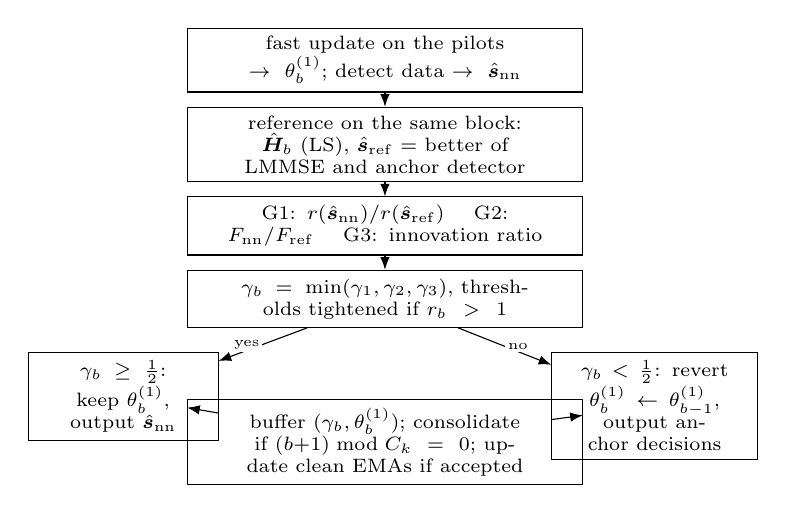
\begin{tikzpicture}[node distance=1.8mm]
\node[box,text width=48mm] (a) {fast update on the pilots $\to\theta^{(1)}_b$; detect data $\to\hat{\bm s}_{\rm nn}$};
\node[box,text width=48mm,below=of a] (b) {reference on the same block: $\hat{\bm H}_b$ (LS), $\hat{\bm s}_{\rm ref}$ = better of LMMSE and anchor detector};
\node[box,text width=48mm,below=of b] (c) {G1: $r(\hat{\bm s}_{\rm nn})/r(\hat{\bm s}_{\rm ref})$ \quad G2: $F_{\rm nn}/F_{\rm ref}$ \quad G3: innovation ratio};
\node[box,text width=48mm,below=of c] (d) {$\gamma_b=\min(\gamma_1,\gamma_2,\gamma_3)$, thresholds tightened if $r_b>1$};
\node[box,text width=22mm,below left=3mm and -4mm of d] (e) {$\gamma_b\ge\tfrac12$: keep $\theta^{(1)}_b$,\\ output $\hat{\bm s}_{\rm nn}$};
\node[box,text width=24mm,below right=3mm and -4mm of d] (f) {$\gamma_b<\tfrac12$: revert $\theta^{(1)}_b\leftarrow\theta^{(1)}_{b-1}$,\\ output anchor decisions};
\node[box,text width=48mm,below=9mm of d] (g) {buffer $(\gamma_b,\theta^{(1)}_b)$; consolidate if $(b{+}1)\bmod C_k=0$; update clean EMAs if accepted};
\draw[arr] (a)--(b); \draw[arr] (b)--(c); \draw[arr] (c)--(d);
\draw[arr] (d)--(e) node[midway,lbl,left]{yes}; \draw[arr] (d)--(f) node[midway,lbl,right]{no};
\draw[arr] (e)--(g); \draw[arr] (f)--(g);
\end{tikzpicture}
\caption{Decision inside one block.}
\label{fig:gateflow}
\end{figure}

\section{Guarantees}\label{sec:theory}
We state the guarantees for the algorithm as implemented; the full proofs are in the
theory document of the repository. Let $\Phi(\theta;\bm Y,a)$ be the block adaptation map
(the fast state after one block, given the pilots and the anchor), and consider paired
runs on the same clean sequence with and without an attack, with displacements
$d_b=\norm{\theta^{(1),\rm adv}_b-\theta^{(1),\rm clean}_b}$ and $D_k(b)$ for level $k$.

\begin{lemma}[consolidation is a convex combination]\label{lem:convex}
Eq.~\eqref{eq:consol} writes the new level-$(k{+}1)$ state as a convex combination of its
old state and the buffered level-$k$ states, with total weight $s\le\eta^{(k+1)}$ on the
latter. Consequently, if the paired runs have equal verdicts, $D_{k+1}\le\max\{D_{k+1}^{\rm
old},\max_j D_k(j)\}$, and by induction $D_k(b)\le\max_{j\le b}d_j$ for every $k\ge2$.
\end{lemma}
\begin{theorem}[retention certificate]\label{thm:cert}
Let an attack occupy a window of $W$ blocks with equal gate verdicts in the paired runs,
let $n(W)\le\lceil W/C_K\rceil$ be the number of level-$K$ consolidations inside it and
$\Delta_f(W)=\max_{\rm window}d_b$ the largest paired fast-level displacement. Then
\begin{equation}\label{eq:cert}
D_K(W)\le\Delta_f(W)\Big(1-(1-\eta^{(K)})^{n(W)}\Big)\le\eta^{(K)}\Delta_f(W)\,n(W).
\end{equation}
If moreover $\norm{\Phi(\theta;\bm Y+\bm E,a)-\Phi(\theta;\bm Y,a)}\le G_\Phi\norm{\bm E}$ and
$\Phi$ is $L_\theta$- and $L_a$-Lipschitz in $\theta$ and $a$ with $L=L_\theta+L_a<1$, then
$\Delta_f(W)\le G_\Phi\epsilon\min\{1,(1-L_\theta)n_W\}/(1-L)$, where $n_W=\rho_{\rm
blk}(1-p^{\rm rej})W$ counts the attacked blocks the gate accepts; and if $L\le1$ only
(non-expansive), $\Delta_f(W)\le G_\Phi\epsilon\,n_W$.
\end{theorem}
\begin{proof}[Proof sketch]
Level $K$ consolidates $n(W)$ times in the window; each time, by Lemma~\ref{lem:convex},
$D_K\leftarrow(1-s)D_K+s\Delta_f$ with $s\le\eta^{(K)}$, which iterated from $D_K=0$ gives
\eqref{eq:cert}. For the second part, the triangle inequality on $\Phi$ gives $d_b\le
L_\theta d_{b-1}+L_a\max_{k\ge2}D_k(b-1)+G_\Phi\epsilon\chi_b$ with $\chi_b=1$ on attacked
accepted blocks; with the lemma and the geometric sum this solves to the stated bound,
and with $L\le1$ the same inequality is non-expansive and adds at most $G_\Phi\epsilon$ per
accepted attacked block.
\end{proof}
The first part of Theorem~\ref{thm:cert} needs no regularity of the fast learner: the
slow level's exposure is divided by its period whatever the fast level does. The second
part says where the gate enters, through $n_W$, and why rejected blocks inject nothing
(they are reverted). The proposal-level form $\eta^{(K)}\rho\,\epsilon\,G(1-p^{\rm
rej})W/C_K$ holds with $G=G_\Phi/(1-L)$, the Lipschitz constant of the whole block
adaptation rather than of a single gradient.

\begin{theorem}[corruption-robust dynamic regret]\label{thm:regret}
Let $\ell_b$ be $G_\ell$-Lipschitz in $\theta$ and $R_T(u)=\sum_b\ell_b(\theta_b)-\ell_b(u_b)$
the dynamic regret against a comparator sequence. Under the hypotheses of
Theorem~\ref{thm:cert}, $R^{\rm adv}_T(u)\le R^{\rm clean}_T(u)+G_\ell\,T\,\Delta_f(T)$; without
the anchor ($L_a=0$), $R^{\rm adv}_T(u)\le R^{\rm clean}_T(u)+G_\ell G_\Phi\epsilon\,n_T/(1-L_\theta)$;
and a detector that uses level $k$ pays at most
$G_\ell\Delta_f(T)\min\{T,\eta^{(k)}T^2/(2C_k)\}$.
\end{theorem}
The adversary's contribution is additive to the clean regret, linear in the number of
accepted corrupted blocks and divided by the level period. We claim no rate for the clean
term of the full-MLP receiver and report it empirically; for a last-layer-adaptable
(convex) variant the $O(\sqrt{T(1+P_T)})$ dynamic-regret bound of
\cite{zinkevich2003,mokhtari2016} applies with the bounded step \eqref{eq:eta}.

\begin{proposition}[CRC gate]\label{prop:crc}
With i.i.d. symbol errors of probability $p$ in a sub-block of $L$ symbols and an $r$-bit
CRC whose syndrome is uniform on error, $P(\mathrm{pass}\mid p)=(1-p)^L+2^{-r}(1-(1-p)^L)$.
Inverting at $F_{\rm ref}$ gives $p_{\rm ref}$, and the rule ``reject if $F_{\rm nn}/F_{\rm
ref}<\tau_2$'' with
\begin{equation}\label{eq:tau2}
\tau_2=\Big(\frac{1-p_{\rm ref}-\delta}{1-p_{\rm ref}}\Big)^{L},\qquad\delta=\max\{\delta_{\min},\rho\,p_{\rm ref}\},
\end{equation}
rejects exactly when the fast level's error probability exceeds the reference's by more
than $\delta$, up to the Hoeffding fluctuation $2e^{-2nt^2}$ of the pass fraction over $n$
sub-blocks \cite{hoeffding1963}.
\end{proposition}
With $n=781$ the gate is deterministic for practical purposes against any attacker that
raises the SER by more than $\delta$; an attacker that does not has caused less than
$\delta$ of harm. The absolute rule ($\delta\equiv0.01$, our first version) is $30\times$
the clean SER at a $3\cdot10^{-4}$ operating point; the relative rule with $\rho=1$ and
$\delta_{\min}=2\cdot10^{-3}$ (five standard deviations of the pass fraction) follows the
operating point.

\begin{proposition}[residual gate under model mismatch]\label{prop:g1}
Write $\bm y_n=\hat{\bm H}\bm s_n+\bm\nu_n+\bm m_n$ with $\bm m_n$ the model-mismatch term.
For decisions with error pattern $\bm e_n$, $r=\mathrm{mean}\norm{\hat{\bm H}\bm e_n}^2+
\mathrm{mean}\norm{\bm\nu_n+\bm m_n}^2+O(N_d^{-1/2})$, so the ratio
$r(\hat{\bm s}_{\rm nn})/r(\hat{\bm s}_{\rm ref})$ is monotone in the excess decision-error
energy of the fast level and the mismatch only compresses it toward one.
\end{proposition}

\begin{table}[t]
\centering\caption{Constants of Theorem~\ref{thm:cert} measured by finite differences on
clean blocks of the A3 configuration (maximum over 10 blocks and 3 random probes; means
in parentheses). Script: \texttt{certificate\_check.py}.}\label{tab:constants}
\scriptsize
\begin{tabular}{@{}lccccc@{}}
\toprule
$\lambda$ & $G_\Phi$ & $L_\theta$ & $L_a$ & $L_\theta+L_a$ & $\epsilon$ (A3)\\
\midrule
0.5 (default) & 5.21 (3.13) & 0.86 (0.76) & 0.35 (0.32) & 1.20 & 1.05\\
1 & 1.54 (1.43) & 0.54 (0.52) & 0.54 (0.53) & 1.08 & 1.11\\
2 & 2.22 (1.97) & 0.40 (0.35) & 0.82 (0.80) & 1.22 & 1.11\\
4 & 2.21 (2.06) & 0.38 (0.29) & 1.01 (0.99) & 1.39 & 1.11\\
\bottomrule
\end{tabular}
\end{table}
Table~\ref{tab:constants} gives the measured constants. $L_\theta+L_a$ stays near one at
every proximal weight: what the fast map forgets about its own past ($1-L_\theta$) it
inherits from the anchor ($L_a$), because the proximal step drives $\theta$ toward the
anchor. The joint system is non-expansive rather than contractive, so the part of
Theorem~\ref{thm:cert} we claim for the default receiver is the structural bound
\eqref{eq:cert} with the measured $\Delta_f$, checked in Section~\ref{sec:cert}; the
contraction branch is stated for completeness and is not certified by these probes. The
same table shows that $\lambda=1$ cuts the fast level's input sensitivity $G_\Phi$ from
$5.2$ to $1.5$: a stronger prior makes the per-block fit less steerable by the pilots.

\section{Experimental Setup}\label{sec:setup}
A fair test needs strong attackers, the receivers of the literature, several channel
families and many seeds, with every receiver seeing the same realisation.
Table~\ref{tab:scen} lists the scenarios.

\begin{table}[t]
\centering\caption{Evaluation scenarios (all with 3 seeds; E3 and E2 at 10\,dB with 5).}
\label{tab:scen}
\scriptsize
\begin{tabular}{@{}llll@{}}
\toprule
Id & Channel & Attacker & Sweep\\
\midrule
E2 & SED cosine / Jakes 0.05 / $\tanh$ PA / COST2100 & none & SNR 4--16\,dB\\
E3 & SED cosine, 10\,dB & A1 white-box, transfer; jamming & SIR $-10$ to $10$\,dB\\
E3snr & SED cosine & A1 white-box, SIR 0 & SNR 4--16\,dB ($\Delta_{\rm dB}$)\\
E3nl / E3cost & $\tanh$ PA / COST2100 & A1 white-box & SIR $-10$ to $10$\,dB\\
E4 & Jakes 0.05 & A2 targeted, SIR 0 & G3 on / off\\
E5 & SED cosine, 400 blocks & A3, 5\% energy, 300 blocks & $C_K\in\{8,32,128\}$, paired clean run\\
E7 & SED cosine, 10\,dB & gate-aware, weight 5 / 50 / 500 & gate subsets\\
E8 & SED cosine, $8\times8$ & A1 white-box & SIR $-10/0/10$\,dB\\
E9 & Jakes 0.01 / 0.05 / 0.10 & A1 white-box, SIR 0 & Doppler\\
Ablation & SED cosine, 10\,dB & A1 white-box, SIR 0 & 16 variants\\
\bottomrule
\end{tabular}
\end{table}

\textit{Baselines.} LMMSE on the least-squares pilot estimate (no adaptation, the
model-based reference); online DeepSIC \cite{shlezinger2021}; Meta-DeepSIC
\cite{raviv2023}; a drift-detection receiver that adapts only when a $z$-test on the
pilot loss fires (the ``adapt less'' strategy); a MedBN-style receiver that replaces the
adaptation gradient by a median of means over four pilot groups \cite{medbn}; and a
single-memory Titans receiver, the same delta-rule fast learner and surprise rate with
$K=1$ and no gates \cite{behrouz2025titans}, which isolates the memory hierarchy from the
fast rule. All DeepSIC-type receivers share the architecture, the pre-training and the
300 adaptation steps per block of Table~\ref{tab:setup}.

\textit{Protocol.} Every receiver is run on the same channel realisation, noise and
attack draw for a given seed (paired design); the attacker re-crafts its perturbation
for each victim. We report means over seeds; for the main cells we add 95\% bootstrap
confidence intervals over the (seed, block) pairs (10\,000 resamples \cite{efron1993}) and
two-sided Wilcoxon signed-rank tests \cite{wilcoxon1945} on the paired per-block
differences, Holm-corrected within each table \cite{holm1979}. The attack window, the
recovery criterion and the budget definition were fixed before the sweeps; the one
change made after seeing results, the relative CRC slack, is reported with its first,
failed calibration (Section~\ref{sec:cost2100}).

\section{Results}\label{sec:results}
We compare all receivers under the availability attack, look at the gate's side of the
same runs, vary the SNR, test significance, then stress the receiver with the targeted,
boiling-frog and gate-aware attackers, check the certificate, dissect the receiver, and
test its transfer to other channels, a larger system and faster fading.

\subsection{Main Comparison}
\begin{table*}[t]
\centering\caption{SER in the attack window (blocks 30--69) under A1 at SIR
$-10/-5/0/5/10$\,dB, $4\times4$ SED channel, 10\,dB, mean over seeds (5 for online, Meta
and Citadel, 3 otherwise). Pre: blocks 0--29. Post and recovery at SIR 0\,dB (30: not
within the run). LMMSE has no adaptation map; its attacked row is the transfer one.
Script: \texttt{sweep.py e3}, \texttt{analyze.py}.}\label{tab:main}
\scriptsize
\begin{tabular}{@{}lcccccccc@{}}
\toprule
Receiver & Pre & White-box A1: $-10$ / $-5$ / $0$ / $5$ / $10$\,dB & Post & Rec. & Transfer A1: $-10$ / $-5$ / $0$ / $5$ / $10$\,dB & Rec. & Jamming $0$\,dB\\
\midrule
LMMSE & 0.056 & -- & -- & -- & 0.873 / 0.740 / 0.447 / 0.149 / 0.064 & 0 & 0.892\\
Online DeepSIC & 0.071 & 0.973 / 0.938 / 0.772 / 0.475 / 0.277 & 0.088 & 11 & 0.352 / 0.357 / 0.347 / 0.295 / 0.210 & 10 & 0.855\\
Meta-DeepSIC & 0.062 & 0.861 / 0.805 / 0.593 / 0.400 / 0.241 & 0.186 & 30 & 0.195 / 0.201 / 0.213 / 0.211 / 0.175 & 14 & 0.851\\
Drift-detection & 0.077 & 0.975 / 0.942 / 0.776 / 0.459 / 0.265 & 0.097 & 10 & 0.345 / 0.359 / 0.337 / 0.277 / 0.199 & 7 & 0.858\\
MedBN-style & 0.065 & 0.933 / 0.853 / 0.738 / 0.549 / 0.397 & 0.204 & 30 & 0.724 / 0.641 / 0.544 / 0.423 / 0.296 & 30 & 0.858\\
Single-memory Titans & 0.068 & 0.975 / 0.939 / 0.788 / 0.486 / 0.276 & 0.075 & 6 & 0.363 / 0.368 / 0.354 / 0.290 / 0.200 & 6 & 0.861\\
\midrule
Citadel-Rx (proposed) & \textbf{0.040} & \textbf{0.026 / 0.025 / 0.028 / 0.030 / 0.034} & \textbf{0.029} & \textbf{0} & \textbf{0.025 / 0.025 / 0.027 / 0.030 / 0.037} & \textbf{0} & 0.848\\
\bottomrule
\end{tabular}
\end{table*}

\begin{figure*}[t]
\centering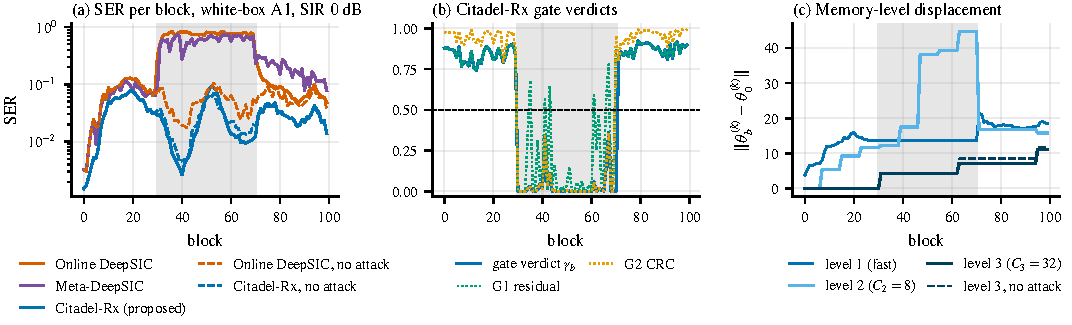
\includegraphics[width=\textwidth]{fig_run}
\caption{One run (seed 0, white-box A1 at SIR 0\,dB, shaded window). (a) SER per block;
dashed: the same receiver without attack. (b) Citadel-Rx gate verdicts: the CRC gate drops
to zero on every poisoned block and the combined verdict rejects it. (c) Displacement of
the three memory levels from their pre-trained value; level 2 absorbs the reverted fast
states' weights and returns, level 3 follows its no-attack trajectory.}
\label{fig:run}
\end{figure*}

\begin{figure*}[t]
\centering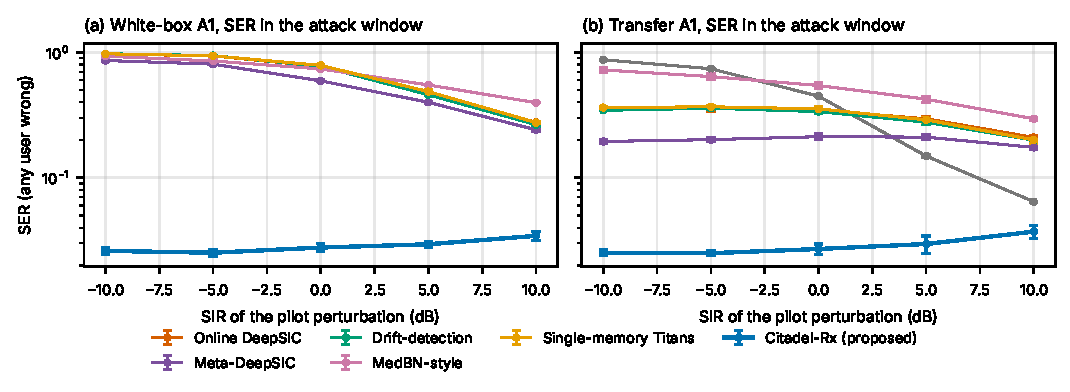
\includegraphics[width=\textwidth]{fig_sir}
\caption{SER in the attack window against the attacker's budget, (a) white-box and (b)
transfer A1; markers are seed means, bars the seed standard deviation. Script:
\texttt{fig\_paper.py}.}
\label{fig:sir}
\end{figure*}

Table~\ref{tab:main} and Figs.~\ref{fig:run}--\ref{fig:sir} give the main result. Under
the white-box attack every baseline is destroyed at SIR $\le0$\,dB (SER $0.59$--$0.98$)
and still loses $4$--$6\times$ at $10$\,dB; Meta-DeepSIC and the MedBN-style receiver do
not recover within 30 blocks (post-attack SER $0.19$--$0.20$ against $0.06$--$0.07$
before), reproducing the observation of \cite{wu2024}. The transfer attack is weaker for
the baselines ($0.20$--$0.36$) but not harmless, and wrecks LMMSE at high budgets. The
jamming control makes the point a security reviewer wants: against every baseline,
poisoning 200 pilot bits costs as much as jamming 50\,000 data bits with the same energy
($0.77$ against $0.86$ at 0\,dB) and, unlike jamming, leaves persistent damage.

Against Citadel-Rx the attack is worthless at every budget and under both knowledge
models: the attack-window SER ($0.025$--$0.037$) is at or below the receiver's own clean
level in those blocks (Fig.~\ref{fig:run}a: the window covers the easy part of the
fade, so the honest comparison is with the dashed no-attack curve, from which the
attacked run is indistinguishable), recovery is immediate, and the slow memory follows
its no-attack trajectory (Fig.~\ref{fig:run}c). The attacker is reduced to jamming, which
costs continuous power and leaves no trace. Before the attack, Citadel-Rx is $44\%$
below online DeepSIC ($0.040$ against $0.071$); Section~\ref{sec:clean} examines that
gain.

\subsection{The Gate's Side}
\begin{table}[t]
\centering\caption{Gate statistics of Citadel-Rx in the runs of Table~\ref{tab:main}:
rejection rate of poisoned blocks / false-rejection rate of clean blocks, and the area
under the ROC of the verdict as a detector (pooled over seeds and budgets).}
\label{tab:gate}
\scriptsize
\begin{tabular}{@{}lccccc@{}}
\toprule
Attacker & $-10$\,dB & $-5$\,dB & $0$\,dB & $5$\,dB & $10$\,dB\\
\midrule
White-box A1 & 0.98 / 0.013 & 0.98 / 0.007 & 0.97 / 0.003 & 0.95 / 0.000 & 0.86 / 0.000\\
Transfer A1 & 0.99 / 0.013 & 0.99 / 0.017 & 0.97 / 0.003 & 0.94 / 0.000 & 0.78 / 0.000\\
\midrule
AUC of $\gamma$ (A1, pooled) & \multicolumn{5}{c}{0.989 (G1 alone 0.986, G2 alone 0.999, G3 alone 0.967)}\\
Jamming control & \multicolumn{5}{c}{rejection 1.00, false rejection 0.000, AUC 1.000}\\
\bottomrule
\end{tabular}
\end{table}
Table~\ref{tab:gate} views the same runs from the gate. Rejection falls with the
attacker's budget ($0.98\to0.86$) because a weak perturbation does less damage and more
often stays inside the CRC slack; the blocks it leaks cost little, which is why the SER
column of Table~\ref{tab:main} rises only from $0.026$ to $0.034$. False rejections are at
most $1.7\%$. The CRC gate is the strongest single detector of the availability attack
(AUC $0.999$), the residual gate is close, and the prior gate is weak against A1 as
designed. Under data jamming the residual ratio is inverted (the fast level's decisions
fit the model better than the reference's; AUC $0.117$ for G1 alone) and the CRC gate
carries the verdict alone: the gates are not interchangeable, and $\gamma=\min$ inherits
the best of them.

\subsection{Degradation Across SNR}
\begin{figure*}[t]
\centering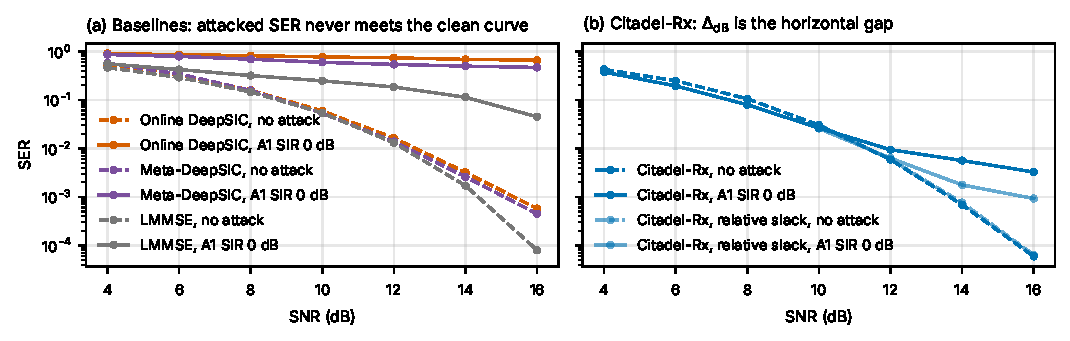
\includegraphics[width=\textwidth]{fig_snr}
\caption{SER against SNR without attack (dashed) and under white-box A1 at SIR 0\,dB
(solid), 3 seeds. (a) For every baseline the attacked curve never meets the clean one on
the grid, so $\Delta_{\rm dB}$ is unbounded. (b) Citadel-Rx with the absolute and the
relative CRC slack. Script: \texttt{fig\_paper.py}.}
\label{fig:snr}
\end{figure*}
Fig.~\ref{fig:snr} reports the degradation metric of \cite{wu2024}. For every baseline the
attacked SER stays at $0.45$--$0.91$ over the whole $4$--$16$\,dB grid, so the extra SNR
needed to recover the clean SER exceeds the grid everywhere. For Citadel-Rx,
$\Delta_{\rm dB}\le0$ from $4$ to $10$\,dB and $\approx0$ at $12$\,dB with the relative
slack ($0.0062$ attacked against $0.0059$ clean); at $14$ and $16$\,dB the attacked window
sits at $0.0018$ and $0.0009$ against clean $0.0008$ and $0.0001$. This is the honest limit
of the defence: it holds the receiver near $10^{-3}$ under attack; it does not preserve a
$10^{-4}$ operating point, because the $5$--$10\%$ of poisoned blocks that pass the gate
set the floor. Closing it needs a rejection rate of one, not a different slack.

\subsection{Significance and Seed Spread}
\begin{table}[t]
\centering\caption{Paired comparison on (seed, block) pairs in the attack window:
Citadel-Rx minus baseline, 95\% bootstrap interval, Holm-corrected Wilcoxon $p$. Full
tables for every cell: \texttt{docs/STATS.md}.}\label{tab:paired}
\scriptsize
\begin{tabular}{@{}lccc@{}}
\toprule
Citadel-Rx vs. & $\Delta$SER, white-box 0\,dB & $\Delta$SER, clean cosine 10\,dB & $p_{\rm Holm}$\\
\midrule
Online DeepSIC & $-0.745$ [$-0.757$, $-0.731$] & $-0.029$ [$-0.030$, $-0.028$] & $<0.001$\\
Meta-DeepSIC & $-0.565$ [$-0.583$, $-0.546$] & $-0.023$ [$-0.024$, $-0.021$] & $<0.001$\\
Drift-detection & $-0.750$ [$-0.764$, $-0.734$] & $-0.035$ [$-0.037$, $-0.033$] & $<0.001$\\
MedBN-style & $-0.712$ [$-0.736$, $-0.686$] & $-0.034$ [$-0.036$, $-0.032$] & $<0.001$\\
Single-memory Titans & $-0.761$ [$-0.776$, $-0.745$] & $-0.023$ [$-0.025$, $-0.021$] & $<0.001$\\
LMMSE & $-0.420$ [$-0.432$, $-0.409$] (transfer) & $-0.024$ [$-0.025$, $-0.022$] & $<0.001$\\
\bottomrule
\end{tabular}
\end{table}
\begin{table}[t]
\centering\caption{Headline cells with five seeds: mean $\pm$ standard deviation over
seeds.}\label{tab:seeds}
\scriptsize
\begin{tabular}{@{}lccc@{}}
\toprule
Cell & Online DeepSIC & Meta-DeepSIC & Citadel-Rx\\
\midrule
Clean, cosine 10\,dB & $0.0590\pm0.0008$ & $0.0527\pm0.0008$ & $\mathbf{0.0302\pm0.0004}$\\
Clean, Jakes 0.05, 10\,dB & $0.0128\pm0.0058$ & $0.0115\pm0.0050$ & $\mathbf{0.0059\pm0.0028}$\\
A1 white-box, SIR $-10$ & $0.973\pm0.003$ & $0.861\pm0.009$ & $\mathbf{0.026\pm0.002}$\\
A1 white-box, SIR $0$ & $0.772\pm0.013$ & $0.593\pm0.011$ & $\mathbf{0.028\pm0.002}$\\
A1 white-box, SIR $10$ & $0.277\pm0.005$ & $0.241\pm0.006$ & $\mathbf{0.034\pm0.003}$\\
A1 transfer, SIR $0$ & $0.347\pm0.013$ & $0.213\pm0.012$ & $\mathbf{0.027\pm0.003}$\\
Jamming, 0\,dB & $0.855\pm0.001$ & $0.851\pm0.001$ & $0.848\pm0.001$\\
\bottomrule
\end{tabular}
\end{table}
Differences of a few SER points need a significance test. Table~\ref{tab:paired} compares
like with like: every pair of receivers sees the same channel, noise and attack draw, and
the per-block differences are tested with Holm correction over the six comparisons of
each cell. Every difference in Tables~\ref{tab:main} and \ref{tab:clean} is significant
at $p<0.001$, and the intervals exclude zero by a wide margin. Table~\ref{tab:seeds} adds
the spread over five training seeds: the seed standard deviation of Citadel-Rx's attacked
SER is $0.002$--$0.003$, two orders of magnitude below the effect; the Jakes clean cell
spreads for every receiver because the realised fade differs by seed, and the ranking is
the same in all five.

\subsection{Clean Performance}\label{sec:clean}
\begin{table}[t]
\centering\caption{SER without attack, 100 blocks, 3 seeds (5 at 10\,dB cosine/Jakes).
Script: \texttt{sweep.py e2/e2nl/e2cost}, \texttt{analyze.py}.}\label{tab:clean}
\scriptsize
\begin{tabular}{@{}lcccc@{}}
\toprule
Receiver & Cosine 10\,dB & Jakes 10\,dB & $\tanh$ PA 10\,dB & COST2100 8\,dB\\
\midrule
LMMSE & 0.0537 & 0.0095 & 0.0562 & \textbf{0.0041}\\
Online DeepSIC & 0.0590 & 0.0128 & 0.0652 & 0.0096\\
Meta-DeepSIC & 0.0527 & 0.0115 & 0.0595 & 0.0093\\
Drift-detection & 0.0653 & 0.0206 & 0.0691 & 0.0140\\
MedBN-style & 0.0644 & 0.0142 & 0.0605 & 0.0080\\
Single-memory Titans & 0.0529 & 0.0092 & 0.0567 & 0.0102\\
Citadel-Rx (proposed) & \textbf{0.0302} & \textbf{0.0059} & \textbf{0.0331} & 0.0047\\
\bottomrule
\end{tabular}
\end{table}
A defence is only useful if it costs nothing when there is no attack. Citadel-Rx costs
less than nothing on three of the four channel families (Table~\ref{tab:clean}): it is the
best receiver at every SNR from $4$ to $12$\,dB on the cosine, Jakes and nonlinear
channels, halving the SER of online DeepSIC at 10\,dB. Pre-training does not explain it
(pre-trained online DeepSIC: $0.074$ against $0.069$ in the pre-attack blocks), nor does
the fast rule alone (single-memory Titans: $0.053$); Section~\ref{sec:ablate} attributes it
to the proximal anchor, i.e. to the slow memory acting as a prior for a fit from 100
pilot symbols. On COST2100, a nearly diagonal $4\times4$ channel on which LMMSE is close to
optimal, Citadel-Rx matches LMMSE within $2$--$15\%$ at $4$--$8$\,dB while every DeepSIC
baseline is $1.5$--$2.3\times$ worse than LMMSE; the clean gain is channel-dependent and nil
where interference cancellation has nothing to cancel.

\subsection{Targeted, Boiling-Frog and Gate-Aware Attackers}
\begin{table}[t]
\centering\caption{Stress attackers, SER in the attack window (3 seeds; E7 cells with
weight 50 and 500 have 1 seed). Rej.: rejection of poisoned blocks.}\label{tab:stress}
\scriptsize
\begin{tabular}{@{}llccc@{}}
\toprule
Attacker & Receiver & Pre & Window & Rej.\\
\midrule
A2 targeted, Jakes 0.05, 0\,dB & Online DeepSIC & 0.019 & 0.438 & --\\
 & Meta-DeepSIC & 0.017 & 0.350 (post 0.053, rec. 23) & --\\
 & Citadel-Rx, G1+G2 & 0.010 & 0.010 & 0.82\\
 & Citadel-Rx, G1+G2+G3 & 0.010 & 0.010 & 0.83\\
\midrule
Gate-aware, 10\,dB & Citadel-Rx, no gates & 0.039 & 0.531 & 0.00\\
 & G1 only, weight 5 & 0.039 & 0.034 & 0.93\\
 & G1 only, weight 50 & 0.039 & 0.044 & 0.85\\
 & G1 only, weight 500 & 0.039 & 0.074 & 0.30\\
 & G1+G2, weight 5 & 0.039 & 0.024 & 1.00\\
 & G1+G2+G3, weight 5 & 0.039 & 0.026 & 0.99\\
 & G1+G2+G3, weight 500 & 0.039 & 0.027 & 0.95\\
\midrule
A3 boiling frog, 300 blocks & Citadel-Rx, $C_K=8$ & 0.029 & 0.040 (post 0.023) & 0.00\\
 & Citadel-Rx, $C_K=32$ & 0.031 & 0.039 (post 0.023) & 0.00\\
 & Citadel-Rx, $C_K=128$ & 0.032 & 0.039 (post 0.023) & 0.00\\
\bottomrule
\end{tabular}
\end{table}
Table~\ref{tab:stress} stresses the gates. The targeted attacker on a Jakes channel
takes every user of online DeepSIC and Meta-DeepSIC down (window SER $0.44$ and $0.35$; the
$\lambda$-weighted objective is not very selective) while Citadel-Rx stays at its clean
$0.010$ with $82\%$ rejection, with or without the prior gate: G1 and G2 catch this attack
on their own. The gate-aware attacker shows the value of having several gates. Against
the residual gate alone, a large penalty weight halves the rejection rate ($0.93\to0.30$)
at the price of a weaker poison (SER $0.034\to0.074$): evading the residual test costs
poisoning strength, as the design intended, but G1 alone is not enough. Against G1 and G2
together, or all three, the best-effort attacker gains nothing (rejection $0.95$--$1.00$,
SER $0.024$--$0.027$). The boiling-frog attacker passes the gates by construction
(rejection $0$) and buys one SER point over 300 blocks; what it does to the memory is
the subject of the certificate.

\subsection{The Certificate With Measured Constants}\label{sec:cert}
\begin{figure}[t]
\centering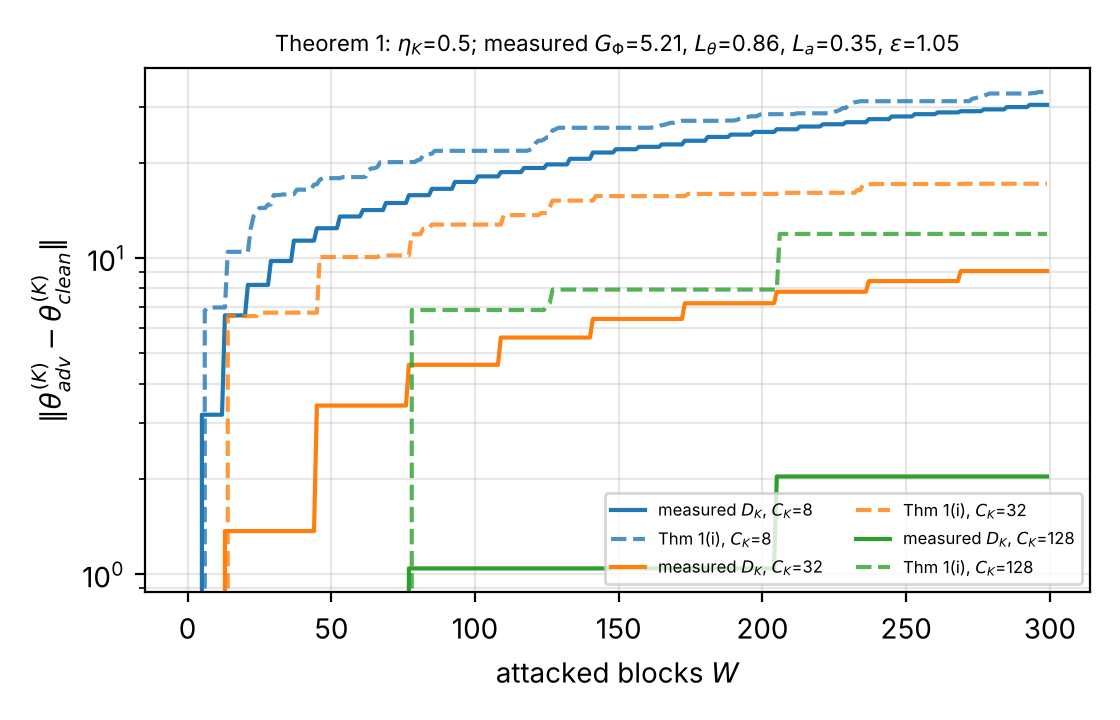
\includegraphics[width=\columnwidth]{fig_e5_certificate_bound}
\caption{Paired displacement of the slowest level under A3 (solid; 3 seeds) and the
structural certificate \eqref{eq:cert} with the measured fast-level displacement
(dashed), for $C_K=8,32,128$ over 300 attacked blocks. Script:
\texttt{certificate\_check.py}.}
\label{fig:cert}
\end{figure}
\begin{table}[t]
\centering\caption{Certificate check on the paired A3 runs ($\eta^{(K)}=0.5$, $p^{\rm
rej}=0$).}\label{tab:cert}
\scriptsize
\begin{tabular}{@{}lccc@{}}
\toprule
$C_K$ & $\Delta_f$ (end of window) & $\max_W D_K(W)/\text{bound}$ & slope of $D_K$ per block\\
\midrule
8 & 33.4 & 0.94 & 0.084\\
32 & 17.2 & 0.53 & 0.029\\
128 & 15.9 & 0.26 & 0.0083\\
\bottomrule
\end{tabular}
\end{table}
Fig.~\ref{fig:cert} and Table~\ref{tab:cert} draw \eqref{eq:cert} against the paired
adversarial/clean trajectories of the slowest level. The bound holds at every $W$ for
every period, is nearly tight at $C_K=8$ (the slow level is then a running average of the
fast level), and the measured slopes scale as $1:0.35:0.10$ against the $1:0.25:0.0625$ of
pure $1/C_K$ ($\propto C_K^{-0.85}$ over a $16\times$ range); the deviation is $\Delta_f$
itself shrinking with $C_K$, because a slower anchor pulls the fast level back harder.
The measured fast displacement ($16$--$34$) is of the size the geometric sum predicts
from $L_\theta$ alone ($\epsilon G_\Phi/(1-L_\theta)\approx39$), i.e. the anchor coupling
does not compound even though $L_\theta+L_a>1$.

\subsection{Ablations}\label{sec:ablate}
\begin{table}[t]
\centering\caption{Ablations under white-box A1 at SIR 0\,dB, 3 seeds (complete receiver
on the same seeds). Script: \texttt{sweep.py ablate}.}\label{tab:ablate}
\scriptsize
\begin{tabular}{@{}lcccc@{}}
\toprule
Configuration & Pre & Window & Rej. & False rej.\\
\midrule
Complete receiver & 0.039 & \textbf{0.028} & 0.97 & 0.003\\
$K=1$ (gates, no slow level) & 0.068 & 0.788 & 0.98 & 0.222\\
$K=2$, $C=(1,8)$ & 0.038 & 0.050 & 0.97 & 0.006\\
$K=4$, $C=(1,4,16,64)$ & 0.038 & 0.029 & 0.97 & 0.011\\
Periods misaligned, $C=(1,3,7)$ & 0.037 & 0.031 & 0.95 & 0.000\\
No gates & 0.039 & 0.540 & 0.00 & --\\
G1 only & 0.039 & 0.031 & 0.97 & 0.000\\
G2 only & 0.039 & 0.028 & 0.97 & 0.000\\
G3 only & 0.039 & 0.507 & 0.08 & 0.000\\
Last layer adaptable & 0.052 & 0.029 & 0.98 & 0.011\\
Plain GD fast rule & 0.066 & 0.048 & 0.90 & 0.072\\
Adam without delta decay & 0.040 & 0.030 & 0.97 & 0.006\\
Fixed step $\eta$ & 0.040 & 0.027 & 0.97 & 0.011\\
No anchor ($\lambda=0$) & \textbf{0.058} & 0.031 & 0.99 & 0.178\\
Jump re-anchor ($\beta=0.25$) \cite{behrouz2025nested} & 0.058 & 0.031 & 0.97 & 0.150\\
No fallback & 0.040 & \textbf{0.245} & 0.97 & 0.011\\
Keep (not revert) rejected update & 0.040 & 0.025 & 1.00 & 0.017\\
\bottomrule
\end{tabular}
\end{table}
Each component is removed in turn (Table~\ref{tab:ablate}). Three carry the result. The
slow memory: with one level the gates fire but there is nothing uncorrupted to fall back
on and the receiver collapses like online DeepSIC ($0.788$); two levels halve the damage
($0.050$), three remove it. The fallback: reverting a rejected update protects the memory
but leaves the block's data to a poisoned fast level ($0.245$). The proximal anchor: it is
the clean gain ($0.039$ against $0.058$ without it), and the jump re-anchoring of
\cite{behrouz2025nested} is no better than no anchoring; both also raise clean false
rejections to $15$--$18\%$ because the fast level drifts away from the memory it is
compared with. The honest negatives: the delta-rule decay and the surprise-driven step
each buy $2$--$3\%$ of clean SER; period alignment with the coherence structure does not
matter on this channel; G3 is useless against A1, as predicted, its role is A2; and
whether a rejected update is reverted or kept makes no difference once the fallback is
active.

\subsection{Generalisation: Channels, System Size and Doppler}\label{sec:gen}
\begin{table*}[t]
\centering\caption{Transfer to other channels, a larger system and faster fading: SER in
the attack window under white-box A1 (3 seeds; pre-attack SER in parentheses; Citadel-Rx
on COST2100 with the relative slack). Scripts: \texttt{sweep.py e3nl/e3rel/e8/e9}.}
\label{tab:gen}
\scriptsize
\begin{tabular}{@{}lccccccc@{}}
\toprule
 & \multicolumn{2}{c}{$\tanh$ PA, $4\times4$} & \multicolumn{2}{c}{COST2100, $4\times4$} & \multicolumn{2}{c}{SED, $8\times8$} & Jakes $f_DT_b=0.01/0.05/0.10$\\
Receiver & SIR $-10$ & SIR $0$ & SIR $-10$ & SIR $0$ & SIR $-10$ & SIR $0$ & SIR $0$\\
\midrule
LMMSE (transfer) & 0.841 (0.058) & 0.421 & 0.063 (0.0001) & 0.0010 & 0.983 (0.141) & 0.793 & 0.067 / 0.067 / 0.103 (0.015--0.021)\\
Online DeepSIC & 0.973 (0.079) & 0.784 & 0.928 (0.0008) & 0.636 & 0.998 (0.250) & 0.971 & 0.719 / 0.719 / 0.717 (0.017--0.026)\\
Meta-DeepSIC & 0.865 (0.067) & 0.656 & 0.791 (0.0007) & 0.345 & 0.972 (0.220) & 0.934 & 0.496 / 0.501 / 0.531 (0.013--0.026)\\
Drift-detection & 0.973 (0.083) & 0.794 & 0.941 (0.0005) & 0.630 & 0.997 (0.259) & 0.971 & 0.728 / 0.738 / 0.717 (0.023--0.040)\\
MedBN-style & 0.908 (0.069) & 0.706 & 0.744 (0.0002) & 0.505 & 0.995 (0.158) & 0.923 & 0.711 / 0.692 / 0.691 (0.015--0.025)\\
Single-memory Titans & 0.971 (0.075) & 0.799 & 0.917 (0.0011) & 0.627 & 0.998 (0.234) & 0.969 & 0.738 / 0.749 / 0.736 (0.015--0.023)\\
Citadel-Rx (proposed) & \textbf{0.026} (0.042) & \textbf{0.026} & \textbf{0.0011} (0.0003) & \textbf{0.0013} & \textbf{0.080} (0.127) & \textbf{0.080} & \textbf{0.0066 / 0.0069 / 0.0075} (0.007--0.015)\\
Rejection / false rej. & 0.99 / 0.017 & 0.98 / 0.006 & 0.89 / 0.00 & 0.86 / 0.00 & 1.00 / 0.05 & 1.00 / 0.05 & 0.92 / 0.94 / 0.97, 0.006--0.033\\
\bottomrule
\end{tabular}
\end{table*}
Table~\ref{tab:gen} repeats the main comparison on the nonlinear channel, the COST2100
traces, an $8\times8$ system and three Doppler rates. On every one, every baseline is
destroyed at SIR $\le0$\,dB and Citadel-Rx stays at or below its pre-attack level. With
eight users the clean gain grows (Citadel-Rx $0.102$ against LMMSE $0.129$ and online
DeepSIC $0.204$ over 100 clean blocks; interference cancellation matters more),
Meta-DeepSIC and MedBN again never recover (post-attack $0.40$--$0.66$), and false
rejections rise to $3$--$5\%$ because the eight-user fade has deeper per-block dips.
Faster fading raises every receiver's clean SER and the gate's false alarms
($0.6\to3.3\%$), not the attacker's success: Citadel-Rx's attacked SER is flat at $0.007$
over a $10\times$ range of Doppler. Gate AUCs are $0.989$ (nonlinear), $0.988$ (COST2100,
relative slack), $0.985$ ($8\times8$) and $0.996$ (Jakes).

\subsection{COST2100 and the Relative Slack}\label{sec:cost2100}
COST2100 at 10\,dB is the one setting where the first version of the receiver left its
clean trajectory. With the absolute CRC slack ($\delta=0.01$), Citadel-Rx's attack-window
SER was $0.0022/0.0032/0.0054/0.0122/0.0111$ at SIR $-10$ to $10$\,dB against a clean
$0.0003$: $50$--$400\times$ better than online DeepSIC, but with rejection falling to
$0.64$, because a one-point slack is $30\times$ the clean SER and the attacker can pass G2
while doing damage. The relative slack of \eqref{eq:tau2} brings the window to
$0.0011/0.0012/0.0012/0.0015/0.0028$ (rejection $0.89/0.90/0.86/0.74/0.40$, no false
rejections) and leaves the linear grid unchanged ($0.025$--$0.029$, rejection
$0.93$--$1.00$, false rejection $\le2\%$). A first calibration with a floor of $10^{-3}$ had
fixed COST2100 but raised linear false rejections to $15$--$20\%$, because the floor sat
inside the statistical resolution of the pass fraction; the floor of $2\cdot10^{-3}$ is
five standard deviations of it. One further honest observation from this channel: LMMSE
attacked through the surrogate is itself nearly immune here ($0.0010$ at SIR 0\,dB), so
on a nearly diagonal channel Citadel-Rx matches, rather than beats, the model-based
receiver under attack ($0.0013$; paired difference $+0.0003$, interval $[-0.0005,+0.0010]$).

\subsection{Cost}
Per block on one CPU worker of the evaluation workstation (eight single-thread workers
in parallel, 300 adaptation steps): LMMSE $0.07$\,s, online DeepSIC $4.0$\,s,
drift-detection $9.2$\,s, Meta-DeepSIC $12.4$\,s, Citadel-Rx $12.2$\,s, single-memory
Titans $14.4$\,s, MedBN-style $37.2$\,s. Citadel-Rx costs $3.1\times$ online DeepSIC and the
same as Meta-DeepSIC; its overhead over the single-memory receiver is the gate (one LMMSE
detection and one CRC check of the data block), while the levels cost memory ($K$ copies
of $15\,628$ parameters), not compute. The white-box attacker spends $3.2$\,s of PGD per
poisoned block.

\section{Discussion}\label{sec:discussion}
Some conclusions are firmer than others; we state what the evidence supports, what it
does not, and what bounds the findings.

Against the attacks of \cite{wu2024} and their stronger variants, the receiver's
robustness is not in doubt: the attacked SER equals the clean one across budgets,
knowledge models, channel families, system sizes and Doppler rates, with intervals and
tests that leave no room for a seed artefact. The mechanism is visible in the records:
the CRC gate drops to zero on poisoned blocks, the fast update is reverted, the data are
detected with the slow memory, and the slow memory follows its no-attack trajectory. The
ablation says which parts matter (the slow level, the fallback, and G1 or G2) and which
do not (period alignment, the delta decay, the surprise rate, reverting versus keeping a
rejected update). We state this plainly because it is the finding most likely to be
misread: the value of the receiver is in its memory and its fallback, not in a cleverer
fast learner.

The clean gain is a second contribution but a conditional one. It is large where
interference cancellation matters (a $44$--$50\%$ lower SER than online DeepSIC on the
SED channel, more with eight users) and nil on a nearly diagonal channel where LMMSE is
already near optimal; the ablation attributes it to the proximal anchor, i.e. to a prior
learned across blocks, which is why the jump re-anchoring of nested learning does not
produce it.

The certificate is the structural bound \eqref{eq:cert} with a measured fast-level
displacement; it holds at every window length and shows the $1/C_K$ mechanism. The
contraction branch of Theorem~\ref{thm:cert} is not certified for the default receiver:
the measured $L_\theta+L_a$ is above one at every proximal weight, and we found this to be
structural rather than a probe artefact. A reader who wants a guarantee with no
measured quantity needs a fast learner that is a contraction jointly in its state and
its anchor, which the present design is not.

Two limits are stated as such. First, at clean SER near $10^{-4}$ the attacked window
sits near $10^{-3}$: the few poisoned blocks that pass the gate set a floor, and a
different slack does not move it; a second-chance re-detection of accepted blocks would.
Second, the CRC gate needs CRC-framed data; in a system where the receiver sees only
uncoded symbols, G1 and G3 remain and, by Table~\ref{tab:ablate}, G1 alone defeats the
non-adaptive attacker but not the gate-aware one.

The remaining assumptions bound the generality of the results. \emph{Threat model:} the
attacker perturbs the received pilots within an energy budget and knows the pilots; a
jammer with a directional array or a spoofer of the data part are outside the model.
\emph{Channel:} block fading with the synthetic, Jakes and COST2100 families of the DeepSIC
literature; no link-level simulation with a 3GPP channel model and LDPC coding was run.
\emph{Modulation:} QPSK with 100 pilot symbols per user. \emph{Receiver:} DeepSIC; the
levels and gates are agnostic to the per-user network, but no other backbone was tested.
\emph{Compute:} the gate's reference detector and CRC check cost one LMMSE pass per
block; the levels cost memory.

\section{Conclusion}\label{sec:conclusion}
We presented a DeepSIC receiver that keeps its adaptable parameters at three time-scales,
consolidates from fast to slow memory only through blocks that pass three label-free
physics-consistency tests, pulls the fast level toward the slow projection, and detects a
rejected block with the slow memory. Against the pilot-poisoning attacks that destroy
online and meta-learned receivers, the attacked symbol error rate equals the clean one
at every budget, on four channel families, two system sizes and three Doppler rates, with
$86$--$99\%$ of poisoned blocks rejected and at most $1.7\%$ of clean ones; without attack
the receiver halves the error rate of online DeepSIC where interference cancellation
matters. The slow memory's exposure to a bounded attack is divided by its period and
multiplied by the gate's miss rate, and the bound holds with measured constants. Two
lessons follow. First, the defence is in the memory, not in the learner: a single
test-time memory with the same fast rule is as vulnerable as online DeepSIC. Second, a
gate tied to the attacker's own objective (the CRC) is what a gate-aware attacker cannot
evade without giving that objective up.

Several directions follow from the limits stated above: a re-detection pass for accepted
blocks to lift the $10^{-3}$ floor at high SNR; a fast learner that is a joint
contraction, so that the certificate's second branch becomes measurable; link-level
simulation with LDPC coding and a 3GPP channel model, where the CRC gate becomes the
transport-block CRC; and other backbones (DeepRx-style convolutional receivers), where
the levels and gates apply unchanged.

\section*{Data and Code Availability}
Code, configuration files, all 1\,926 run records, the statistics and the scripts that
regenerate every table, figure and number of this paper are available at
\url{https://github.com/abraheemrashid99-sys/Citradel-Rx}. The COST2100 traces are those
released with \cite{raviv2023}.

\begin{thebibliography}{40}
\bibitem{oshea2017} T.~O'Shea and J.~Hoydis, ``An introduction to deep learning for the physical layer,'' \emph{IEEE Trans. Cogn. Commun. Netw.}, vol.~3, no.~4, pp. 563--575, Dec. 2017.
\bibitem{honkala2021} M.~Honkala, D.~Korpi, and J.~M.~J. Huttunen, ``DeepRx: Fully convolutional deep learning receiver,'' \emph{IEEE Trans. Wireless Commun.}, vol.~20, no.~6, pp. 3925--3940, Jun. 2021.
\bibitem{samuel2019} N.~Samuel, T.~Diskin, and A.~Wiesel, ``Learning to detect,'' \emph{IEEE Trans. Signal Process.}, vol.~67, no.~10, pp. 2554--2564, May 2019.
\bibitem{shlezinger2023} N.~Shlezinger, J.~Whang, Y.~C. Eldar, and A.~G. Dimakis, ``Model-based deep learning,'' \emph{Proc. IEEE}, vol.~111, no.~5, pp. 465--499, May 2023.
\bibitem{shlezinger2021} N.~Shlezinger, R.~Fu, and Y.~C. Eldar, ``DeepSIC: Deep soft interference cancellation for multiuser MIMO detection,'' \emph{IEEE Trans. Wireless Commun.}, vol.~20, no.~2, pp. 1349--1362, Feb. 2021.
\bibitem{raviv2023} T.~Raviv, S.~Park, O.~Simeone, Y.~C. Eldar, and N.~Shlezinger, ``Online meta-learning for hybrid model-based deep receivers,'' \emph{IEEE Trans. Wireless Commun.}, vol.~22, no.~10, pp. 6415--6431, Oct. 2023.
\bibitem{wu2024} K.~Wu, W.~Jiang, D.~Niyato, Y.~Li, and C.~Luo, ``Transfer-based adversarial poisoning attacks for online (MIMO-)deep receivers,'' arXiv:2409.02430, Sep. 2024.
\bibitem{wu2023tta} T.~Wu, F.~Jia, X.~Qi, J.~T. Wang, V.~Sehwag, S.~Mahloujifar, and P.~Mittal, ``Uncovering adversarial risks of test-time adaptation,'' in \emph{Proc. Int. Conf. Mach. Learn. (ICML)}, 2023.
\bibitem{medbn} H.~Park, J.~Hwang, S.~Mun, S.~Park, and J.~Ok, ``MedBN: Robust test-time adaptation against malicious test samples,'' in \emph{Proc. IEEE/CVF Conf. Comput. Vis. Pattern Recognit. (CVPR)}, 2024.
\bibitem{blanchard2017} P.~Blanchard, E.~M. El~Mhamdi, R.~Guerraoui, and J.~Stainer, ``Machine learning with adversaries: Byzantine tolerant gradient descent,'' in \emph{Adv. Neural Inf. Process. Syst. (NeurIPS)}, 2017.
\bibitem{steinhardt2017} J.~Steinhardt, P.~W. Koh, and P.~Liang, ``Certified defenses for data poisoning attacks,'' in \emph{Adv. Neural Inf. Process. Syst. (NeurIPS)}, 2017.
\bibitem{lykouris2018} T.~Lykouris, V.~Mirrokni, and R.~Paes Leme, ``Stochastic bandits robust to adversarial corruptions,'' in \emph{Proc. ACM Symp. Theory Comput. (STOC)}, 2018.
\bibitem{behrouz2025nested} A.~Behrouz, M.~Razaviyayn, P.~Zhong, and V.~Mirrokni, ``Nested learning: The illusion of deep learning architectures,'' in \emph{Adv. Neural Inf. Process. Syst. (NeurIPS)}, 2025.
\bibitem{behrouz2025titans} A.~Behrouz, P.~Zhong, and V.~Mirrokni, ``Titans: Learning to memorize at test time,'' arXiv:2501.00663, 2025.
\bibitem{finn2017} C.~Finn, P.~Abbeel, and S.~Levine, ``Model-agnostic meta-learning for fast adaptation of deep networks,'' in \emph{Proc. Int. Conf. Mach. Learn. (ICML)}, 2017.
\bibitem{madry2018} A.~Madry, A.~Makelov, L.~Schmidt, D.~Tsipras, and A.~Vladu, ``Towards deep learning models resistant to adversarial attacks,'' in \emph{Proc. Int. Conf. Learn. Represent. (ICLR)}, 2018.
\bibitem{zinkevich2003} M.~Zinkevich, ``Online convex programming and generalized infinitesimal gradient ascent,'' in \emph{Proc. Int. Conf. Mach. Learn. (ICML)}, 2003.
\bibitem{mokhtari2016} A.~Mokhtari, S.~Shahrampour, A.~Jadbabaie, and A.~Ribeiro, ``Online optimization in dynamic environments: Improved regret rates for strongly convex problems,'' in \emph{Proc. IEEE Conf. Decis. Control (CDC)}, 2016.
\bibitem{hoeffding1963} W.~Hoeffding, ``Probability inequalities for sums of bounded random variables,'' \emph{J. Amer. Statist. Assoc.}, vol.~58, no.~301, pp. 13--30, 1963.
\bibitem{jakes1974} W.~C. Jakes, \emph{Microwave Mobile Communications}. New York, NY, USA: Wiley, 1974.
\bibitem{liu2012cost} L.~Liu, C.~Oestges, J.~Poutanen, K.~Haneda, P.~Vainikainen, F.~Quitin, F.~Tufvesson, and P.~De~Doncker, ``The COST 2100 MIMO channel model,'' \emph{IEEE Wireless Commun.}, vol.~19, no.~6, pp. 92--99, Dec. 2012.
\bibitem{ts38212} 3GPP, ``NR; Multiplexing and channel coding,'' TS 38.212, 2024.
\bibitem{efron1993} B.~Efron and R.~J. Tibshirani, \emph{An Introduction to the Bootstrap}. New York, NY, USA: Chapman \& Hall, 1993.
\bibitem{wilcoxon1945} F.~Wilcoxon, ``Individual comparisons by ranking methods,'' \emph{Biometrics Bull.}, vol.~1, no.~6, pp. 80--83, 1945.
\bibitem{holm1979} S.~Holm, ``A simple sequentially rejective multiple test procedure,'' \emph{Scand. J. Statist.}, vol.~6, no.~2, pp. 65--70, 1979.
\end{thebibliography}

\begin{IEEEbiographynophoto}{Abraheem Rashid}
is with the Department of Computer Science, Brunel University London, London, U.K.
\end{IEEEbiographynophoto}

\end{document}
